\begin{figure}[!htbp]
\begin{center}
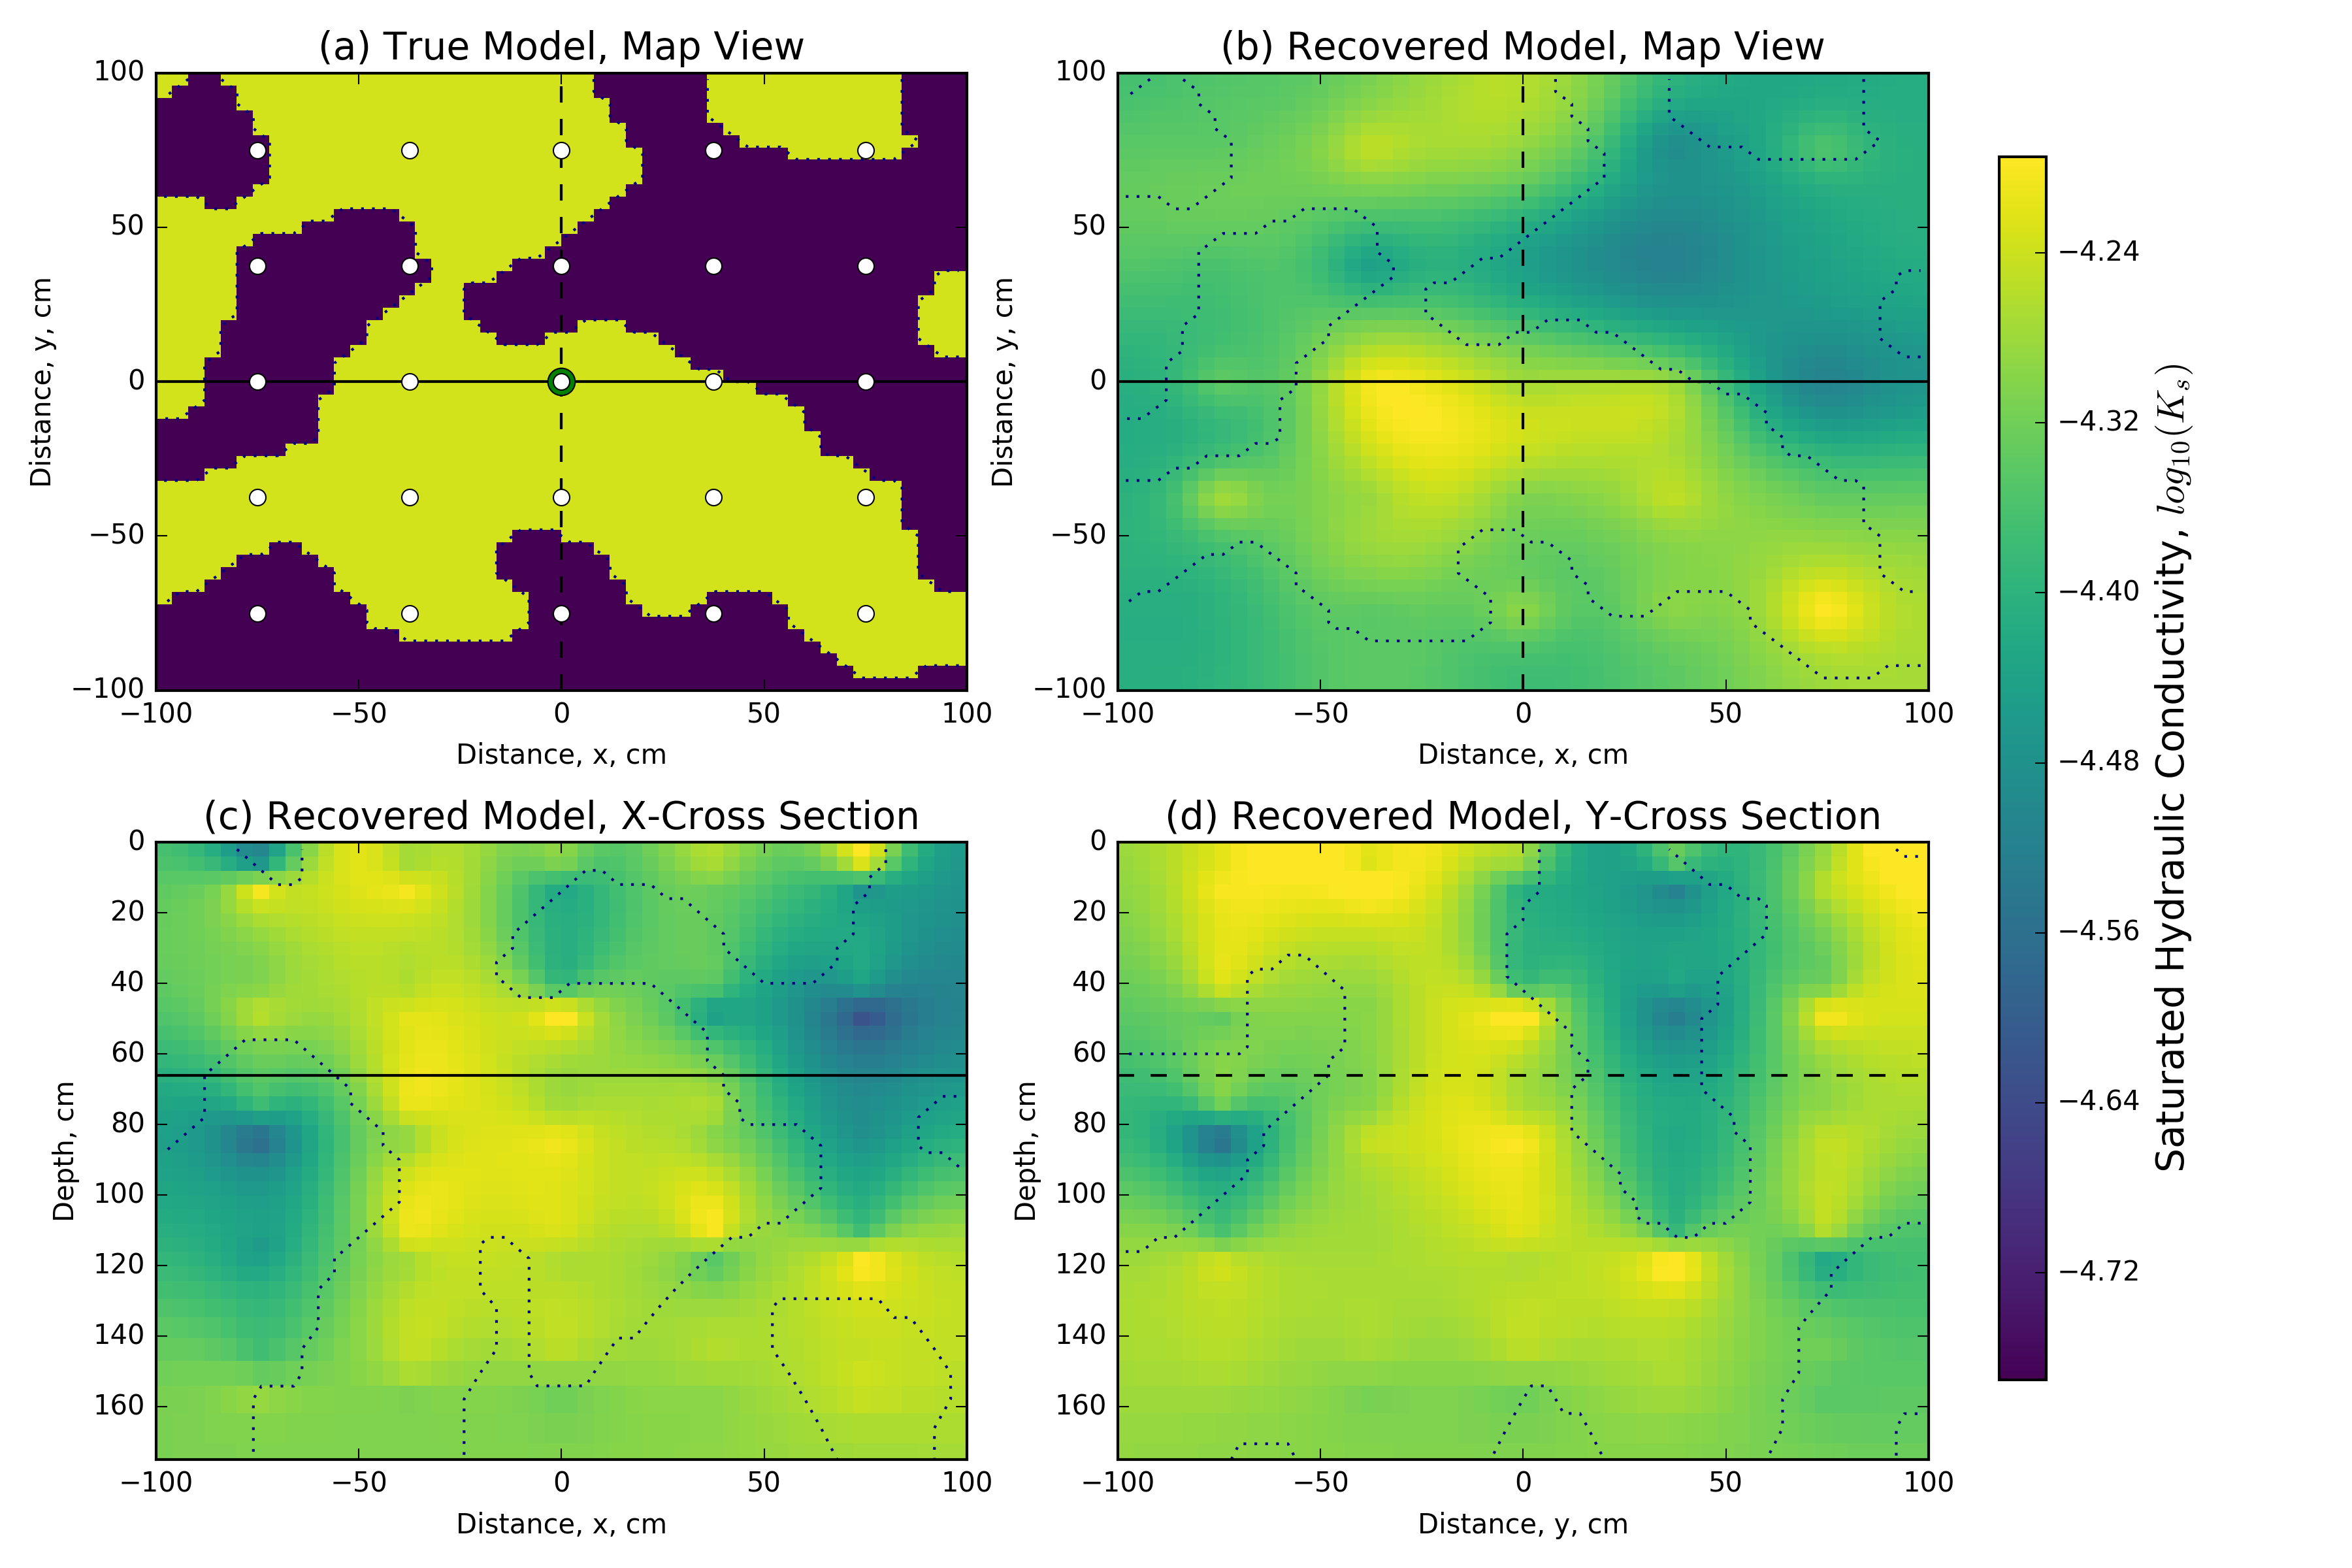
\includegraphics[width=0.9\textwidth]{figures/richards/inversion3d-results.png}
\end{center}
\caption{The 3D distributed saturated hydraulic conductivity model recovered from the inversion compared to the (a) synthetic model map view section, using (b) the same map view section, (c) an X-Z cross section and (d) a Y-Z cross-section. The synthetic model is shown as an outline on all sections, and tie lines are shown on all sections as solid and dashed lines, all location measurements are in centimeters.}
\label{fig:richards-inversion3d-results}
\end{figure}
